% Using KOMA Script document style
% Font size setting and
% option to skip empty lines as new paragraphs
\documentclass[10pt,a4paper]{article}
% Packages without Options
\usepackage{
	algorithm,
	alltt,
	algpseudocode,
	amsfonts,
	amssymb,
	appendix,
	array,
	booktabs,
	dirtree,
	enumitem,
	float,
	footnote,
	gensymb,
	geometry,
	graphicx,
	interval,
	karnaugh-map,
	lipsum,
	listings,
	longtable,
	makecell,
	mathtools,
	minted,
  nicematrix,
	parskip,
	pdfpages,
	pgfkeys,
	pgfplots,
	subcaption,
	tabularx,
	tablefootnote,
	textcomp,
	tikz,
    titlecaps,
	venndiagram,
	wrapfig,
	wrapfig,
	xcolor
}



% Packages with Options

\usepackage[framemethod=tikz]{mdframed}
\usepackage[colorlinks,linkcolor=cyan, citecolor=cyan, urlcolor=cyan]{hyperref}
\usepackage[labelfont=bf,textfont=it,labelsep=period]{caption}
\usepackage[RPvoltages]{circuitikz}
\usepackage[english]{babel}
\usepackage[nameinlink,noabbrev]{cleveref}

\definecolor{mintedbackground}{rgb}{0.97,0.97,0.97}

\setminted[cpp]{
bgcolor=mintedbackground,
    linenos=true,
    breaklines=true,}

\setminted[js]{
bgcolor=mintedbackground,
    linenos=true,
    breaklines=true,}

\setminted[python]{
bgcolor=mintedbackground,
    linenos=true,
    breaklines=true,}
    

\linespread{1.5}

% Package: AlgorithmicX
% Sets all comments to be indentend and aligned

\renewcommand{\Comment}[2][.7\linewidth]{%
  \leavevmode\hfill\makebox[#1][l]{//~#2}}


% Package: Interval
% Sets the style of mathematical intervals
\intervalconfig{
soft open fences, separator symbol=,,
}

% Package: Geometry
% Sets the page margins
\geometry{
    a4paper,
    left=32mm,
    right=22mm,
    top=22mm,
    }
	
% Creates a proper caption name for algorithms
\newcommand{\algorithmautorefname}{Algorithm}
\newcommand{\listingautorefname}{Listing}
\algrenewcommand{\algorithmiccomment}[1]{\texttt{// #1} }
% Creates a numbered environment for Theorems
\newtheorem{theorem}{Theorem}

% Redefine the implication arrow to be a simple, thin arrow instead of the default, thick arrow
\renewcommand{\implies}{\rightarrow}

% Create a new command for the set complement to make my logical statements easier to read
\newcommand{\compl}{\overline}

% Creates commands for combinatorics nCr and nPr
\newcommand{\nCr}[2]{\,_{#1}C_{#2}} % nCr
\newcommand{\nPr}[2]{\,_{#1}P_{#2}} % nPr

% Package: tikz
% Loads libraries for drawing automata, 
\usetikzlibrary{automata,positioning,shadows,arrows, shapes.gates.logic.US, calc}

% Creates a command to create a button shape
\newcommand*\keystroke[1]{%
  \tikz[baseline= (key.base)]
    \node[%
      draw,
      fill=white,
      drop shadow={shadow xshift=0.25ex,shadow yshift=-0.25ex,fill=black,opacity=0.75},
      rectangle,
      rounded corners=2pt,
      inner sep=1pt,
      line width=0.5pt,
      font=\scriptsize\sffamily
    ] (key) {#1\strut};
}

% Package: pgfplot
% Sets the global options for PGF Plots
\pgfplotsset{compat=newest}

% Package: tikz
% Flowchart Shapes
\tikzstyle{startstop} = [rectangle, rounded corners, minimum width=3cm, minimum height=1cm,text centered, draw=black, fill=red!30]
\tikzstyle{io} = [trapezium, trapezium left angle=70, trapezium right angle=110, minimum width=3cm, minimum height=1cm, text centered, draw=black, fill=blue!30]
\tikzstyle{process} = [rectangle, minimum width=3cm, minimum height=1cm, text centered, draw=black, fill=orange!30]
\tikzstyle{decision} = [diamond, minimum width=3cm, minimum height=1cm, text centered, draw=black, fill=green!30]
\tikzstyle{arrow} = [thick,->,>=stealth]

% Disable Minted syntax error highlights (red boxes)
\AtBeginEnvironment{minted}{%
  \renewcommand{\fcolorbox}[4][]{#4}}

% Listings Style (non-minted)

\lstdefinestyle{arjuncode}{
    basicstyle=\ttfamily,
    breakatwhitespace=false,         
    breaklines=true,                 
    captionpos=b,                    
    keepspaces=true,                 
    numbers=left,                    
    numbersep=5pt,                  
    showspaces=false,                
    showstringspaces=false,
    showtabs=false,                  
    tabsize=2
}

\lstset{style=arjuncode}

\graphicspath{{images/}}


\title{CM1035: Algorithms and Data Structures I\\ Summary}
\author{Arjun Muralidharan}
\begin{document}

\maketitle
\newpage
\tableofcontents
\listoffigures
\listoftables
% \listofalgorithms

\newpage
\renewcommand{\subsubsectionautorefname}{section\negthinspace}

\section{Problems, algorithms and
flowcharts}

\begin{mdframed}
\textbf{Learning Outcomes}
\begin{itemize}[label={\checkmark}]
\item Explain in broad strokes what are  problems and algorithms in Computer Science.
\item Explain the basic elements and construction of flowcharts.
\item Express elements of simple algorithms as flowchart.
\end{itemize}
\end{mdframed}

\subsection{Problems}
A \textbf{computational problem} is a statement of a desired input/output relationship. An \textbf{algorithm} is a tool for solving such a problem, i.e.~a computational procedure for achieving that input/output relationship. A problem is well-defined when there is a clearly stated input and a description of the desired output.

A specific input needed to compute a solution is called an \textbf{instance} of a problem.

Algorithms predate computers and have existed since almost 3000. They are not specific to computer science. Multiple algorithms can solve the same problem. It is therefore important to be able to decide on the best algorithm. A good metric is to check if an algorithm can cover a wide variety of inputs. Another metric is the time it takes to execute an algorithm.

\subsubsection{Heron's Method}
In computation, we are faced the limitation that computers can only store finite numbers. Hence, irrational numbers need to be approximated.
\begin{equation*}
\left|\sqrt{2}-\frac{x}{y}\right| \leq \eta
\end{equation*}
where \(\frac{x}{y}\) is an approximation and \(\eta \) is the remaining error.

Heron's method approximates the value of a square root \(\sqrt{x}\) by the following method.

\begin{enumerate}
  	\item Make a guess \(g\) for the square root of a number \(x\). A good starting point is the \emph{mean} between \(1\) and \(x\). Also define \(n\) as the number of decimal points desired for precision.
	\item Calculate \(\frac{x}{g}\).
	\item If \(\frac{x}{g} - g < 10^{-(n-1)}\), return g. Otherwise, carry on.
	\item Calculate the mean between \( \frac{x}{g}\) and \(g\). Set this to be the new \(g\).
	\item Repeat from step 2.
\end{enumerate}
The flowchart for Heron's algorithm is shown in \autoref{fig:heron}.

\begin{figure}[ht]
\centering
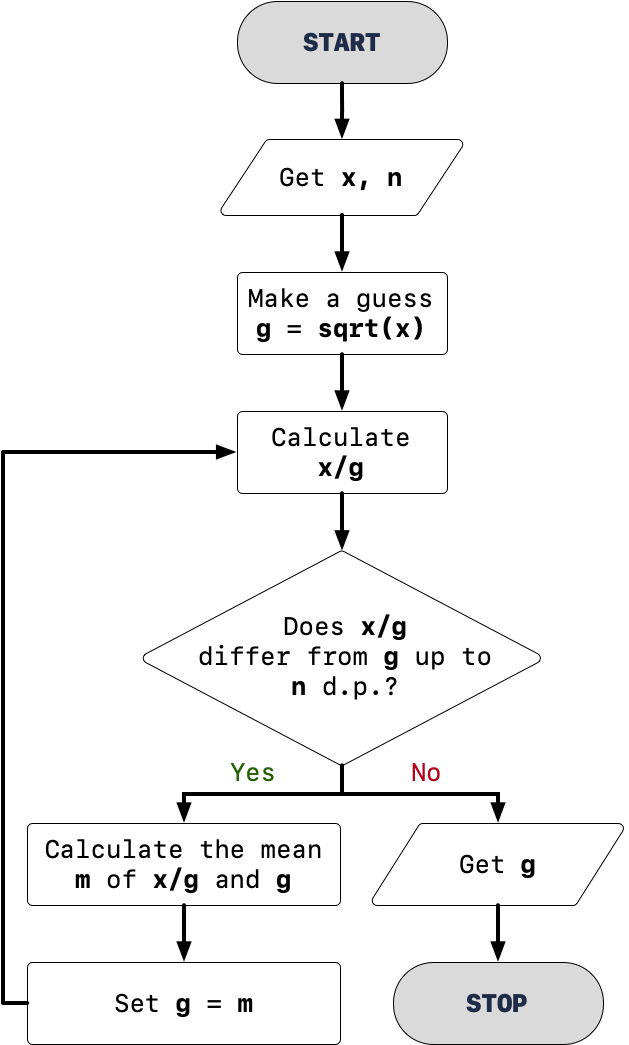
\includegraphics[width=6cm]{heron}
\caption{Heron's Algorithm}\label{fig:heron}
\end{figure}

\subsubsection{Euclid's Algorithm}
Another algorithm is \textbf{Euclid's Algorithm}, which finds the greatest common divisor of two non-zero integers.

The flowchart for Euclid's algorithm is shown in \autoref{fig:euclid}.

\begin{figure}[ht]
\centering
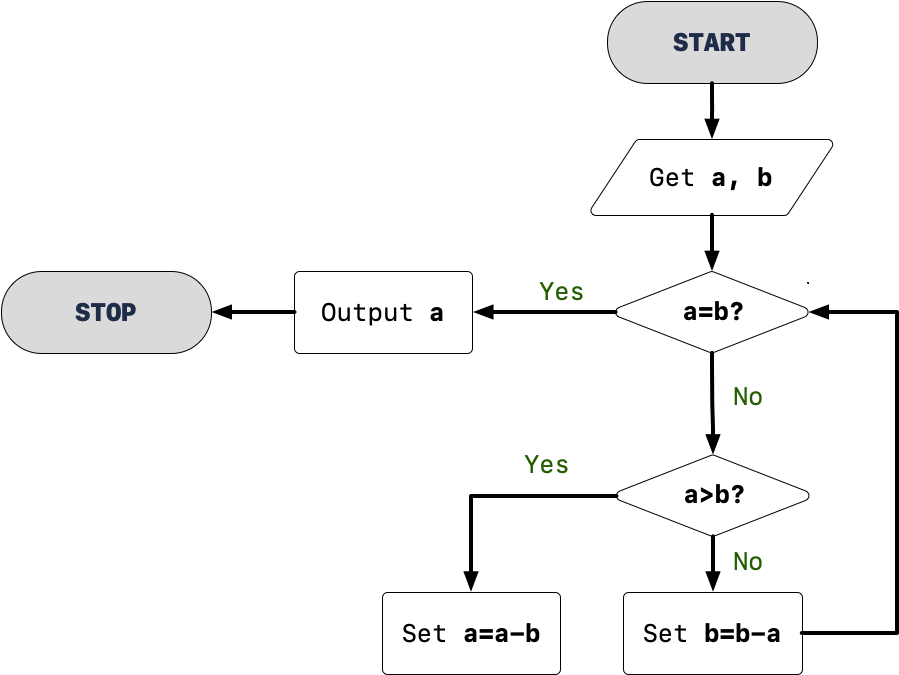
\includegraphics[width=6cm]{euclid}
\caption{Euclid's Algorithm}\label{fig:euclid}
\end{figure}

\section{Pseudocode}

\begin{mdframed}
\textbf{Learning Outcomes}
\begin{itemize}[label={\checkmark}]
\item Explain the necessity and concept of pseudocode.
\item Describe the concept of iteration and how it is represented in pseudocode.
\item Convert flowchart (if possible) to pseudocode

\end{itemize}
\end{mdframed}

Pseudocode allows for notation of an algorithm in a more readable format than flowcharts. You should be able to translate a flowchart into Pseudocode. Further, it allows for abstracting from any specific programming language. The notation for pseudocode is shown in \autoref{tab:pseudo}. An example is shown in \autoref{alg:exp}

\begin{table}[ht]
\centering
\begin{tabular}{p{0.2\textwidth}p{0.7\textwidth}}
\toprule
\textbf{Operator}  & \textbf{Notation} \\ \midrule
Assignment & \( \leftarrow \) \\
Arithmetic &  \(+ \quad - \quad \times \quad / \) \\
Comparison & \(= \quad \neq \quad < \quad > \quad \leq \quad \geq \) \\
Logic & \( \vee \quad \wedge \quad \neg \quad \mathbf{if \ldots then}\) \\
\bottomrule
\end{tabular}
\caption{Notation in Pseudocode}\label{tab:pseudo}
\end{table}

\paragraph{Example} The following algorithm is shown using pseudocode.


\begin{algorithm}[H]
\caption{Simple example of pseudocode}\label{alg:exp}
\begin{algorithmic}
\State{ \( t \leftarrow  18 \) }
\State{ \( T\leftarrow  20 \) }
	\If{\(t < T\)}
		\State{\(t \leftarrow t + 0.5\) }
	\EndIf{}
\end{algorithmic}
\end{algorithm}

\subsection{Functions}
Functions are noted with the \textbf{function} keyword and contains a body. The body is bookended by \textbf{end function}. An example is shown in \autoref{alg:func}.

\begin{algorithm}[H]
	\caption{Functions}\label{alg:func}
	\begin{algorithmic}
		\Function{EVEN}{\emph{n}}
			\If{\(n \mod 2 = 0 \)}
			\State{\textbf{return} true}
			\EndIf{}		
		\EndFunction{}
	\end{algorithmic}
\end{algorithm}


\subsection{Loops}

We generally work with two kinds of loops: \textbf{for} loops and \textbf{while} loops. \textbf{for} loops execute a fixed number of iterations and generally increment a counter for each iteration. \textbf{while} loops execute as long as a certain condition is true.

Loops can be exited using the \textbf{break} or \textbf{continue} statements. However, these should be avoided if possible.

An example of \textbf{for} and \textbf{while} loops are provided in \autoref{alg:loops}.

\begin{algorithm}[H]
	\caption{Loops}\label{alg:loops}
	\begin{algorithmic}
		\State{\(x \leftarrow 1\)}
		\For{\(2 \leq i \leq 10\)}
		\State{\(x \leftarrow x + i\)}
		\EndFor{}
		\State{\(x \leftarrow 1\) }
		\State{\(y \leftarrow 0\)}
		\While{\(x < 11\)}
		\State{\(x \leftarrow x + y\)}
		\EndWhile{}
	\end{algorithmic}
\end{algorithm}

\section{Abstract Data Types \& Structures}

\begin{mdframed}
	\textbf{Learning Outcomes}
	\begin{itemize}[label={\checkmark}]
		\item Describe the basic elements of an abstract data structure
		\item Explain queues, stacks and vectors in terms of their structure and operations
		\item Compare these three different abstract data structures of vectors, stacks and queues
	\end{itemize}
	\end{mdframed}

\subsection{Booleans and Integers}
We have so far already worked with two abstract data types. These are not data structures, as they are not defined by their operations.
\begin{enumerate}
	\item \textbf{Booleans}, which can take the values \textbf{TRUE} and \textbf{FALSE}.
	\item \textbf{Integers}, which can take a value from the set of whole numbers \( \mathbb{N} \).
\end{enumerate}

\subsection{Vectors}
\textbf{Vectors} are an abstract data type and an arrangement of elements with the following properties:

\begin{enumerate}
	\item They have a \emph{fixed} length.
	\item Elements cannot be \emph{deleted}.
	\item Elements cannot be \emph{added}.
	\item All elements can be accessed (using a \( SELECT \) operation).
	\end{enumerate}

	\autoref{tab:vectorops} lists valid operations on a vector.
\begin{table}[ht]
	\centering
	\begin{tabular}{@{}ll@{}}
	\toprule
		Operation & Pseudocode \\ \midrule
	length & \( \textrm{LENGTH}[v] \)  \\
	select[k] & \( v[k] \)  \\
	store![o,k] & \( v[k] \gets o \)  \\
	Construct new vector of length \( n \)  & \( \textrm{\textbf{new} Vector } w(n) \) \\ \bottomrule
	\end{tabular}
	\caption{Vector operations}\label{tab:vectorops}
	\end{table}

We assume that vectors are indexed starting at 1. This is because their length is stored at index 0 of an array.

\subsection{Queues}
A \textbf{queue} is a kind of vector. It is a sequential arrangement of ordered elements, but with the following properties:

\begin{enumerate}
	\item They have a \emph{variable} length.
	\item Elements can only be \emph{deleted} from the \emph{head}.
	\item Elements can only be \emph{added} at the \emph{tail}.
	\item Elements can only be accessed at the head of the queue. To access other elements, first the preceding elements need to be removed from the head the queue.
	\end{enumerate}

	\autoref{tab:queueops} lists valid operations on a queue. A queue follows a \emph{FIFO} (first-in, first-out) policy, meaning that elements added first (and have been in the queue the longest) are accessed first.
\begin{table}[ht]
	\renewcommand{\arraystretch}{2}
	\centering

	\begin{tabular}{@{}ll>{\raggedright\arraybackslash}p{7cm}@{}}
	\toprule
		\textbf{Operation}  & \textbf{Pseudocode}  & \textbf{Description}  \\ \midrule
	head & \( \textrm{HEAD}[q] \) & Returns the element at the head of the queue \\
	dequeue! & \( \textrm{DEQUEUE}[q] \) & Returns and removes the element at the head\\
	enqueue![o] & \( \textrm{ENQUEUE}[o,q] \) & Adds an element to the tail of the queue with the value \( o \) \\
	empty? & \( \textrm{EMPTY}[q] \) & Asks if the queue has any elements, and returns \( \textrm{TRUE} \) if empty\\
	Construct new (empty) queue & \( \textrm{\textbf{new} Queue } q \) & Creates a new, empty stack\\ \bottomrule
	\end{tabular}
	\caption{Queue operations}\label{tab:queueops}
	\end{table}

\subsection{Stacks}
A \textbf{stack} is another kind of vector. It is a sequential arrangement of ordered elements with the following properties:

\begin{enumerate}
	\item They have a \emph{variable} length.
	\item Elements can only be \emph{deleted} from the \emph{top}.
	\item Elements can only be \emph{added} at the \emph{top}.
	\item Elements can only be accessed at the top of the stack. To access other elements, first the preceding elements need to be removed from the top of the stack.
	\end{enumerate}

	\autoref{tab:stackops} lists valid operations on a stack. A stack follows a \emph{LIFO} (last-in, first-out) policy, meaning that elements added most recently (and have been in the queue the shortest amount of time) are accessed first.
\begin{table}[ht]
	\renewcommand{\arraystretch}{2}
	\centering
	\begin{tabular}{@{}ll>{\raggedright\arraybackslash}p{8cm}@{}}
	\toprule
		\textbf{Operation}  & \textbf{Pseudocode}  & \textbf{Description}  \\ \midrule
	push![o] & \( \textrm{PUSH}[o,s] \) & Adds an element to the top of the stack \\
	top & \( \textrm{TOP}[o,s] \) & Returns the element at top of the stack
	\\
	pop! & \( \textrm{POP}[s] \) & Returns and removes the element at the top of the stack\\
	empty? & \( \textrm{EMPTY}[s] \) & Asks if the stack has any elements, and returns \( \textrm{TRUE} \) if empty\\
	Construct new (empty) stack  & \( \textrm{\textbf{new} Stack } q \) & \\ \bottomrule
	\end{tabular}
	\caption{Stack operations}\label{tab:stackops}
	\end{table}

	\section{Data Structures \& Searching Data I}

	\begin{mdframed}
		\textbf{Learning Outcomes}
		\begin{itemize}[label={\checkmark}]
			\item Explain the difference between an abstract data structure and a concrete data structure
			\item Explain how abstract data structures can be implemented by arrays and linked lists
			\item Describe the linear search algorithm
		\end{itemize}
		\end{mdframed}

	\subsection{Arrays}
	An \textbf{array} is a set of elements that a computer can manipulate. Arrays are a way to implement abstract data structures such as vectors, stacks and queues. It is \textbf{not} an abstract data structure, but rather an implementation thereof.

	An array allocates a fixed amount of memory for a given data structure and therefore cannot change in size. This is reflected in the abstract data structure of a vector. An array only has two possible operations since it's size is fixed:

	\begin{enumerate}
		\item \( read[k] \) to access an array element at index \( k \)   
		\item \( write![o,k] \) to write or overwrite the value \( o \) at index \( k \).
	\end{enumerate}

	Arrays are indexed starting at 0. Usually, the length of an abstract data structure (such as a vector) is stored at this index.

	\subsection{Dynamic Arrays}
	
	A \textbf{dynamic array} is an abstract data structure that allows for extensibility. It is similar to the vector with the operations shown in \autoref{tab:dynamicops}.

	\begin{table}[ht]
		\renewcommand{\arraystretch}{2}
		\centering
		\begin{tabular}{@{}ll>{\raggedright\arraybackslash}p{6cm}@{}}
		\toprule
			\textbf{Operation}  & \textbf{Pseudocode}  & \textbf{Array implementation}  \\ \midrule
		length & \( \textrm{LENGTH}[d] \) & read[0]  \\
		select[k] & \( d[k] \) & read[k] \\
		store![o,k] & \( d[k] \leftarrow o \) & write![o,k] \\
		removeAt![k] & \( d[k] \leftarrow \emptyset, k \leq LENGTH[d] \) & write![d[k+1], k], write![,d[length[d]]], write![2,0]\tablefootnote{The first operation shifts the last element to the left by one. Repeat this for further elements on the right to be shifted. The second operation overwrites the last element with an empty value. The third operation updates the array length stored at index \( 0 \).}\\
		insertAt![o,k] & \( d[k] \leftarrow o, k \leq LENGTH[d] + 1 \) & new Array[length[d]+1], write![0,length[d]+1], write! elements on left to old locations, write![o,k], write! elements on right to new locations \\ \bottomrule
		\end{tabular}
		\caption{Dynamic array operations}\label{tab:dynamicops}
	\end{table}

The dynamic array operations are all implementable using an array with its basic \( read \) and \( write \) operations.

\subsection{Linear Search}

A linear search solves the problem of answering whether a specific search term is present on an abstract data structure. It returns either the index at which a search term was found, or false.

In a \emph{vector}, linear search needs to systematically look at all the elements one after the other to determine if the value is in the data structure. A pseudocode implementation of linear search is shown in \autoref{alg:lsvec}.

\begin{algorithm}[H]
	\caption{Linear Search --- \( \mathcal{O}(n) \)}\label{alg:lsvec}
	\begin{algorithmic}
		\Function{LinearSearch}{\emph{v, item}}
		\For{\( 1 \leq i \leq \) LENGTH[v]}
		\If{\( v[i] = item \)}
		\State{\textbf{return} \( i \) }
		\EndIf{}
		\EndFor{}
		\State{\textbf{return} FALSE}
		\EndFunction{}
	\end{algorithmic}
\end{algorithm}

A linear search using \textbf{stacks} or \textbf{queues} needs to prevent data loss.

\begin{enumerate}
	\item For \textbf{stacks}, we \texttt{push} elements to a second vector and then \texttt{pop!} the elements to access elements beneath
	\item For \textbf{queues}, we \texttt{dequeue!} elements and \texttt{enqueue!} them to the end of the queue. In order to prevent an infinite loop, we also first \texttt{enqueue!} a new ``end of queue'' item to the stack, which we check for.  
\end{enumerate}

\subsection{Linked Lists}
The \textbf{linked list} is another data structure that can implement abstract structures.
\paragraph{Pointers} A pointer stores the address of a piece of information in memory. In an array, all data is stored sequentially. In a linked list, this is not the case. Hence, we need pointers to tell us where to look next. We retrieve underlying data from a pointer by \emph{dereferencing} the pointer. 

\paragraph{Nodes} The collection of a \emph{key} and a \emph{pointer} is called a \textbf{node}. A linked list consists of nodes.  

\paragraph{Singly and Doubly Linked} A linked list is \textbf{singly linked} if the nodes only contain a pointer \( x.next \)  to the next node. In a \textbf{doubly linked} list, nodes contain pointers \( x.next \) and \( x.prev \) to additionally point to the previous node.

\paragraph{Head} A special pointer exists in a singly linked list, called the \textbf{head}. This is a pointer that is not associated with a node. If we dereference this pointer, we retrieve the the first node of the linked list.


\paragraph{Tail} The final node has a pointer to \texttt{NULL}. If we see a pointer pointing to the \texttt{NULL} address, we know that we have reached the end of the pointer.

Operations in a linked list cannot access any arbitrary element. Rather, we need to reference elements using pointers.

\begin{enumerate}
	\item \( read[pointer] \) to access a list element at a specific pointer  
	\item \( write![value,pointer] \) to write or overwrite the value at a given pointer.
\end{enumerate}

\paragraph{Searching a Linked List} The best way to search a linked list is to traverse the list with a \emph{temporary pointer} that is initially set to the value \texttt{head}. We can then traverse the list until we find the key or the pointer reads \texttt{NULL}. This algorithm is shown in \autoref{alg:linkedsearch}.

\begin{algorithm}[H]
	\caption{Searching a linked list}\label{alg:linkedsearch}
	\begin{algorithmic}
		\Function{ListSearch}{\emph{L,k}}
		\State{\( x \leftarrow L.head \)}
		\While{\( x \ne \)  NULL and \( x.key \neq k\)}
		\State{\( x \leftarrow x.next \)}
		\EndWhile{}
		\State{\textbf{return} \( x \) }
		\EndFunction{}
	\end{algorithmic}
\end{algorithm}

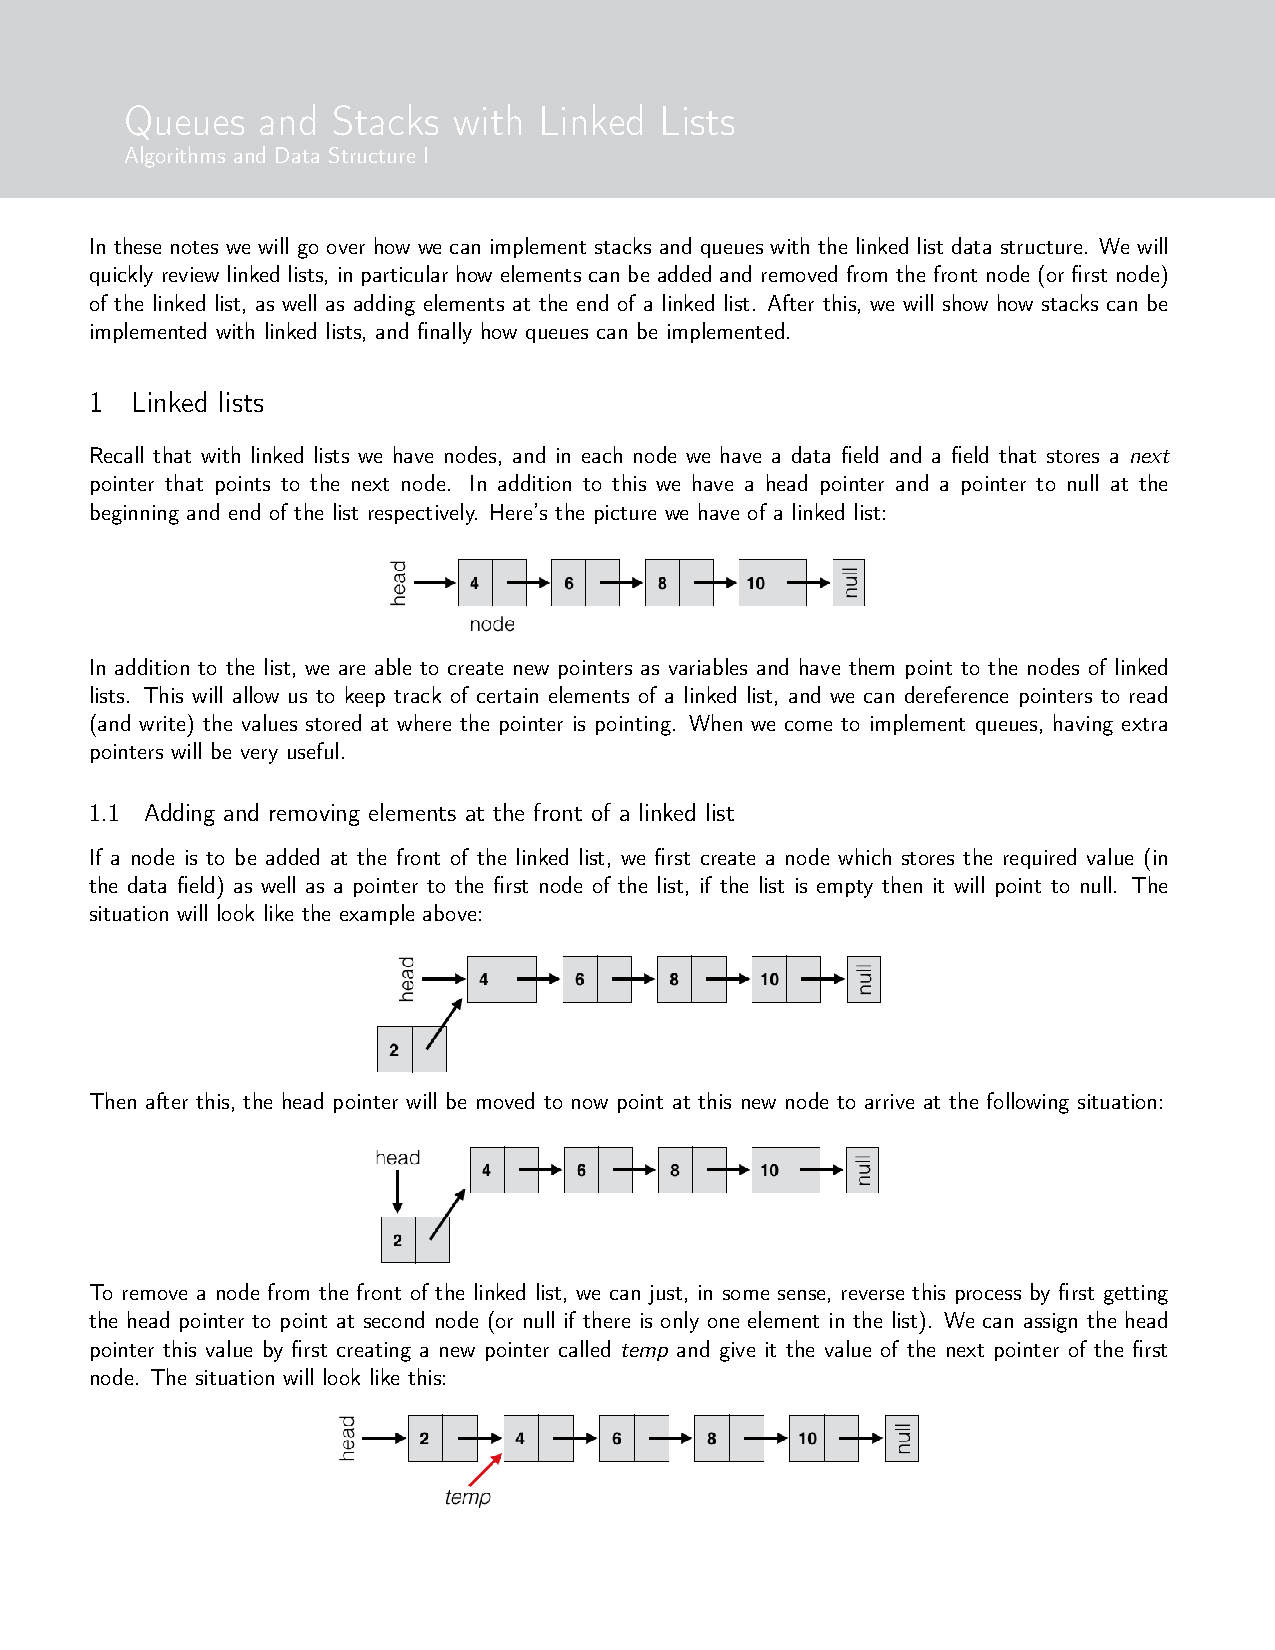
\includepdf[pages=-,frame,templatesize={0.7\textwidth}{0.8\textheight},pagecommand=\thispagestyle{plain}]{linked}

\section{Sorting Data I}
\subsection{Bubble Sort}
Bubble sort is popular, but inefficient, sorting algorithm. It works by repeatedly swapping adjacent elements that are out of order.

It starts at the head of a vector, compares the element to the adjacent elements, and swaps the elements if the first element is larger than the second element.

\paragraph{Passes} The Bubble sort algorithm may need multiple passes to sort the entire vector. The maximum number of passes is given by the most difficult vectors to solve - such that are completely in reverse order. In this case, the number of required passes is \( n-1 \) where \( n \) is the number of elements. Therefore, \textbf{the maximum number of passes required} is always \( n-1 \).  

\begin{algorithm}[H]
	\caption{Bubble Sort --- \( \mathcal{O}(n^2) \) }\label{alg:bubble}
	\begin{algorithmic}
		\Function{Bubblesort}{\emph{vector}}
		\State{\( n \leftarrow\) LENGTH[\( vector \)] }
		\For{\( 1 \leq i \leq n-1 \) }
		\State{\( count \leftarrow 0\) }
		\For{\( 1 \leq j \leq n-1 \)}
		\If{\( vector[j+1] < vector[j] \) }
		\State{Swap(\(vector,j,j+1\))}
		\State{\( count \leftarrow count +1 \) }
		\EndIf{}
		\EndFor{}
		\If{\( count = 0 \) }
		\State{\textbf{break} }
		\EndIf{}
		\EndFor{}
		\State{\textbf{return} \emph{vector} }
		\EndFunction{}
	\end{algorithmic}
\end{algorithm}


\subsection{Insertion Sort}
Insertion sort works from the left of a vector, starting with the second element. It compares the element to the element on the left. If it needs to move, the element is moved along to the left as far as needed.

As an algorithm, we can store the current element in a temporary variable, while we ``move'' elements to the right by overwriting the slots to the right and then restoring the original values from the temporary variable.

\begin{algorithm}[H]
	\caption{Insertion Sort --- \( \mathcal{O}(n^2) \) }\label{alg:insert}
	\begin{algorithmic}
		\Function{InsertionSort}{\emph{v}}
		\For{\( 2 \leq \) LENGTH[v]}
		\State{\( key \leftarrow v[j] \) }
		\State{\( i \leftarrow j - 1 \) }
		\While{\( i > 0 \wedge v[i] > key \) }
		\State{\( v[i+1] \leftarrow v[i] \) }
		\State{\( i \leftarrow i-1 \) }
		\EndWhile{}
		\State{\( v[i+1] \leftarrow key \) }
		\EndFor{}
		\EndFunction{}
	\end{algorithmic}
\end{algorithm}

\section{Random-Access Machines, Growth of Functions and Time Complexity}
\begin{mdframed}
	\textbf{Learning Outcomes}
	\begin{itemize}[label={\checkmark}]
		\item Explain the model of random access machines.
		\item Explain asymptotic growth of functions and worst-case time complexity
		\item Describe worst-case time complexity of bubble and insertion sort
	\end{itemize}
	\end{mdframed}

\subsection{Random Access Machines}
We generally assume a \textbf{random access machine (RAM)} model of computation. In the RAM model, instructions are executed one after another, with no concurrent operations. Memory can be directly access on a memory module.

\begin{itemize}
	\item A RAM generally consists of a \textbf{memory unit} and a \textbf{central processing unit (CPU)}
	\item The CPU consists of a \textbf{program counter} that keeps track of where in the program the computer is, a \textbf{central unit} that is capable of executing \emph{simple arithmetic} and \emph{boolean logic}, and \textbf{registers} that can hold data.
	\item The central unit can \emph{read} input and programs and \emph{write} outputs from and to the memory unit.
	\item The program counter stores a non-negative integer.
	\item The memory unit and registers can store any integer (within the size of the register).
\end{itemize}

\subsection{Worst-Case Time Complexity}

Let \( M \) be a RAM machine that halts on all inputs. The \textbf{running time} or \textbf{time complexity} of \( M \) is the function \( f: N \rightarrow N \), where \( f(n) \) is the maximum number of steps that \( M \) uses on any input of length \( n \) . If \( f(n) \) is the running time of \( M \) , we say that \( M \) runs in time \( f(n) \) and that \( M \) is an \( f(n) \) time random access machine. Customarily we use \( n \) to represent the length of the input.

\subsubsection{Big-O Notation}
The \textbf{running time} of an algorithm on a particular input is the number of steps executed. Machine-independently, we define ``time-steps''. The total running time of an algorithm is defined as
\[
	\textrm{time cost per statement} \times \textrm{no. of executions per statement} = \textrm{total running time}
\]

Function growth can be described and compared using \textbf{Big-O Notation}. In \emph{asymptotic analysis}, we can consider only the highest order terms of a function and ignore the constants. For example, given the function \[
f(n) = 6n^3 + 2n^2 + 20n +45	
\]  

then the \emph{asymptotic} or \emph{Big-O} notation is given as 

\[
	f(n) = \mathcal{O}(n^3)
		\]  
	
A table of common functions and their respective Big-O notation is shown in \autoref{tab:bigo} and sorted by growth rate from slowest to fastest.

\begin{table}[ht]
	\centering
	\begin{tabular}{ll}
	\toprule
	\textbf{Type}  & \textbf{Notation} \\ \midrule
	Constant & \( \mathcal{O}(1) \) \\
	Logarithmic &  \(\mathcal{O}(\log(n)) =\mathcal{O}(\log(n^c))\) \\
	Polylogarithmic & \(\mathcal{O}((\log(n))^c) \) \\
	Linear & \(\mathcal{O}(n) \) \\
	Quadratic & \(\mathcal{O}(n^2) \)  \\
	Polynomial & \(\mathcal{O}(n^c) \) \\
	Exponential & \(\mathcal{O}(c^n) \) \\
	\bottomrule
	\end{tabular}
	\caption{Notation in Pseudocode}\label{tab:bigo}
	\end{table}

Formally, this means that any function is asymptotically \emph{upper-bounded} by its respective Big-O class.

Let \( f \) and \( g \) be functions. It holds that

\[
	\exists k \exists n_0 \forall n \{|f(n)| \leq k \cdot g(n) \mid k > 0, n > n_0  \} \implies f(n) \in \mathcal{O}(g(n))
\]
stating that the size of the function \( f(n) \) will eventually be overtaken by the Big-O class \( g(n) \) multiplied by a constant \( k \). It is an upper bound.

Because Big-O classes live inside each other, we always seek to ascertain the \emph{smallest} Big-O class in which a function exists.

\section{Searching Data II}

\subsection{Binary Search}
Binary Search is a more efficient way of searching an item in a list. It proceeds by halving the list and comparing the middle element to the searched term. If the middle element is smaller than the term, the search continues on the right sublist, and if larger, on the left sublist. Then the procedure is repeated.

\begin{algorithm}[H]
	\caption{Binary Search --- \( \mathcal{O}(\log(n)) \)}\label{alg:binary}
	\begin{algorithmic}
		\Function{BinarySearch}{\emph{v, item}}

		\State{\( L \leftarrow 1\) }
		\State{\( R \leftarrow\) LENGTH\([v]\)}
		\While{\( L \leq R \) }
		\State{\( M \leftarrow \lfloor{\frac{L+R}{2}}\rfloor{} \) }
		\If{\( v[M] < item \) }
		\State{\( L \leftarrow M+1 \) }
		\ElsIf{\( v[M] > item \) }
		\State{\( R \leftarrow M-1 \) }
		\Else{}
		\State{\textbf{return} \( M \) }
		\EndIf{}
		\EndWhile{}
		\State{\textbf{return} false}

		\EndFunction{}
	\end{algorithmic}
\end{algorithm}

Binary search is faster than linear search because each additional search step works on a smaller input (half of the previous input). Hence the time to complete one additional step decreases by half with each step. Hence the algorithm is logarithmic.

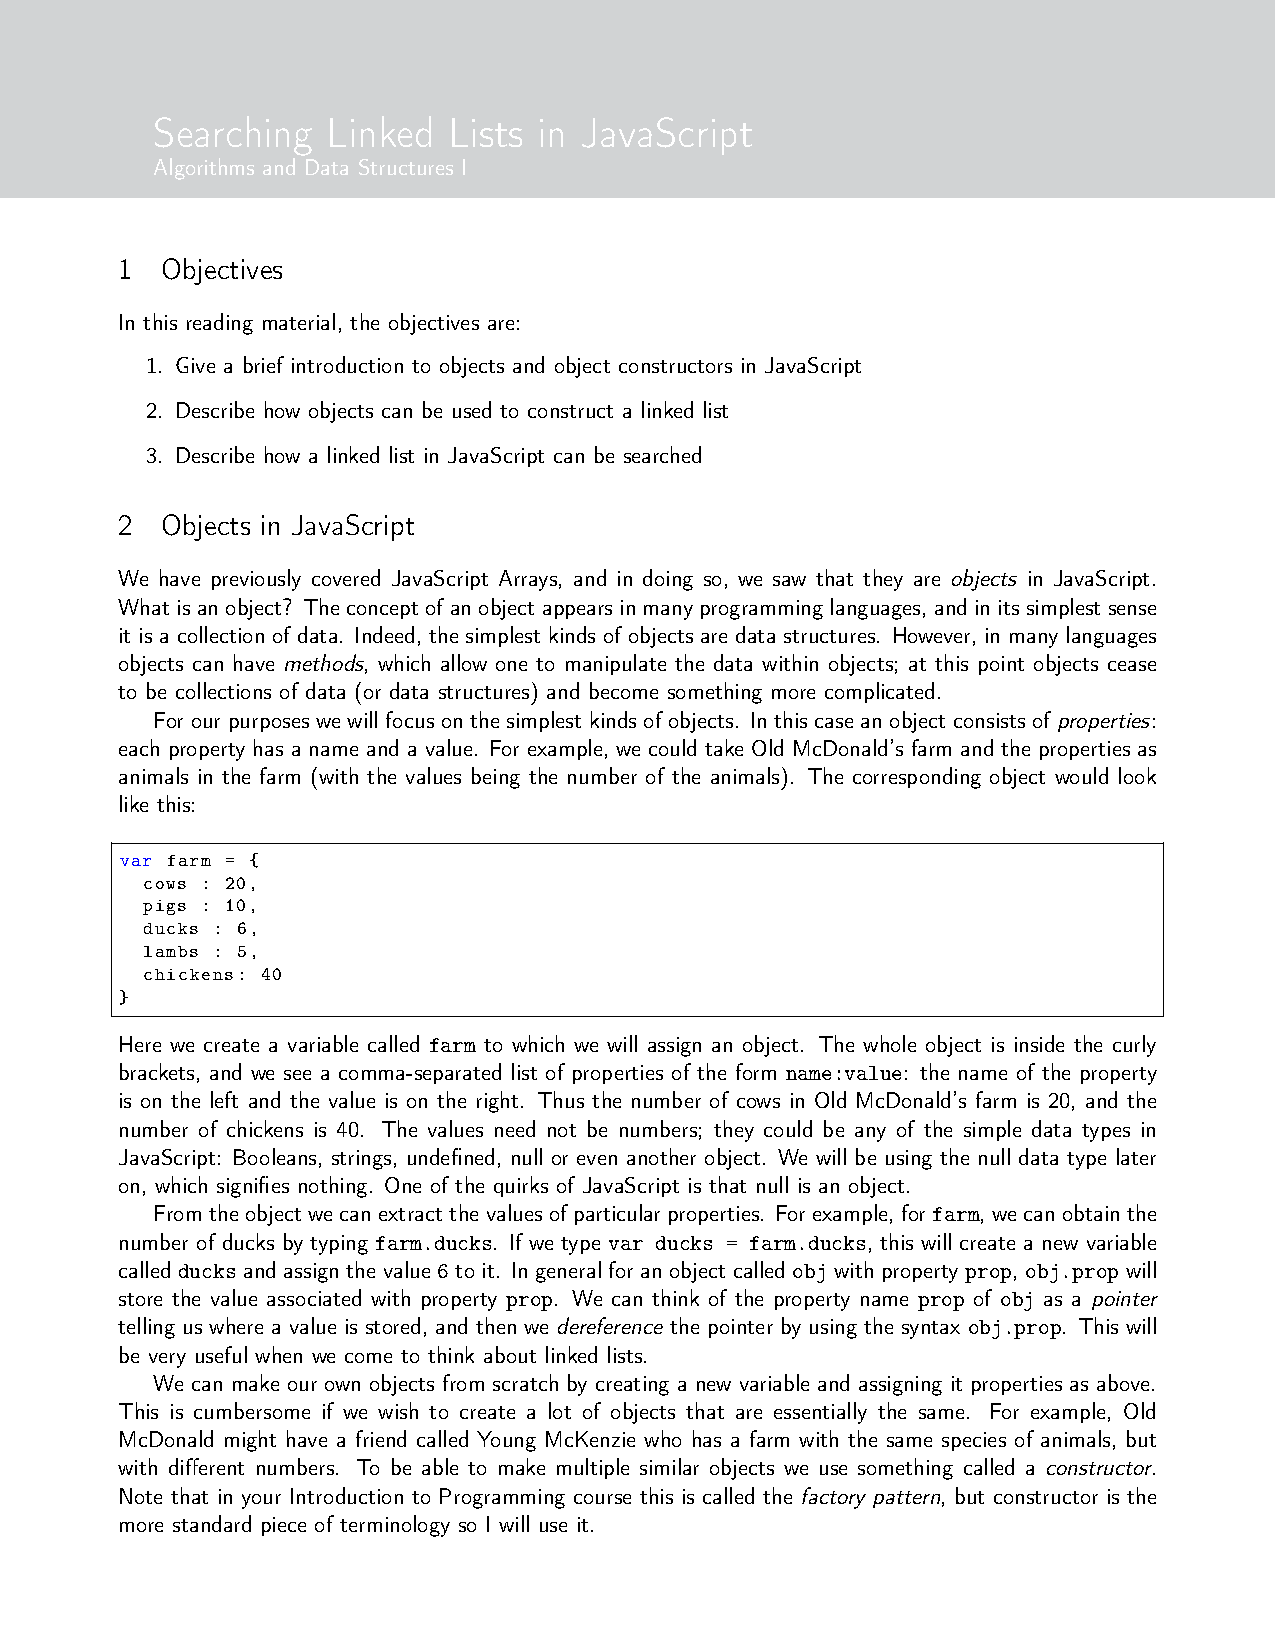
\includepdf[pages=-,frame,templatesize={0.7\textwidth}{0.8\textheight},pagecommand=\thispagestyle{plain}]{linkedSearch}

\section{Recursion}
Recursion is the concept of a procedure referring to itself recursively. The main applications for using recursion are
\begin{itemize}
	\item \textbf{Decrease and conquer}: Decreasing the problem to a \emph{base case} and calling a procedure recursively on every decreasing inputs until the base case is reached. 
	\item \textbf{Divide and conquer}: Split the problem into smaller partial problems and sort those first. 
\end{itemize}

\begin{algorithm}[H]
	\caption{Recursive decrease-and-conquer procedure}\label{alg:fact}
	\begin{algorithmic}
		\Function{Factorial}{\emph{n}}
		\If{\( n=0 \) }
		\State{\textbf{return} 1}
		\EndIf{}
		\State{\textbf{return} \textsc{Factorial}\(( n-1 )\)  }

		\EndFunction{}
	\end{algorithmic}
\end{algorithm}

\subsection{Call Stack}
The call stack is a part of programming languages that is used to manage function calls and variables. At the beginning of a function call, the compiler creates a \textbf{stack frame} to hold all the variables and arguments relevant to that function. Every time a function terminates, the stack is popped and the memory cleared. Each time a function is called, it is pushed on to the stack, and popped when the function terminates. This ensures that function calls happen in order.
If a function has too much recursion, this can cause a \textbf{stack overflow} as the call stack is stored in memory, which is finite. If a function has infinite recursion, stack overflow is guaranteed.

\section{Sorting Data II}
\subsection{Quicksort}
Quicksort is a recursive algorithm to sort a vector. It partitions the vector into sub-vectors at an arbitrary pivot, and then moves the elements smaller than the pivot to the left of it and elements larger to the right, and then moves the pivot element to the correct location in the partition. It then repeats this process recursively on the sub-vectors.

While Quicksort has a worst-case time-complexity of \( \mathcal{O}(n^2) \), this case is unlikely to occur among possible inputs. The typical time complexity, or average-case complexity, is \( \mathcal{O}(n \log(n)) \)

\begin{algorithm}[H]
	\caption{Quicksort --- \( \mathcal{O}(n^2) \) }\label{alg:quick}
	\begin{algorithmic}
		\Function{Quicksort}{\emph{A, p, r}}
		\If{\( p < r \) }
		\State{\( q = \) \textsc{Partition}\( (A,p,r) \)  }
		\State{\textsc{Quicksort}\( (A,p,q-1) \) }
		\State{\textsc{Quicksort}\( (A,q+1,r) \) }
		\EndIf{}	
		\EndFunction{} \\
		\Function{Partition}{\emph{A,p,r}}
		\State{\( x \leftarrow A[r] \) } \Comment{Set the pivot to be the last element}
		\State{\( i \leftarrow p-1 \) } \Comment{Set \( i \) as the divider between elements smaller or bigger than \( x \) }
		\For{j = p \textbf{to} \( r-1 \) } \Comment{Loop through the vector}
		\If{\( A[j] \leq x\) }
		\State{\( i \leftarrow i+1 \) } \Comment{Move  divider to the right to include an element bigger than \( x \) }
		\State{exchange \( A[i] \)  with \( A[j] \) }  \Comment{Move the \( j \)th element to the left partition}
		\EndIf{}
		\EndFor{}
		\State{exchange \( A[i+1] \) with \( A[r] \)  } \Comment{Move the pivot to the right of the divider}
		\EndFunction{}
	\end{algorithmic}
\end{algorithm}

\begin{figure}[H]
	\centering
	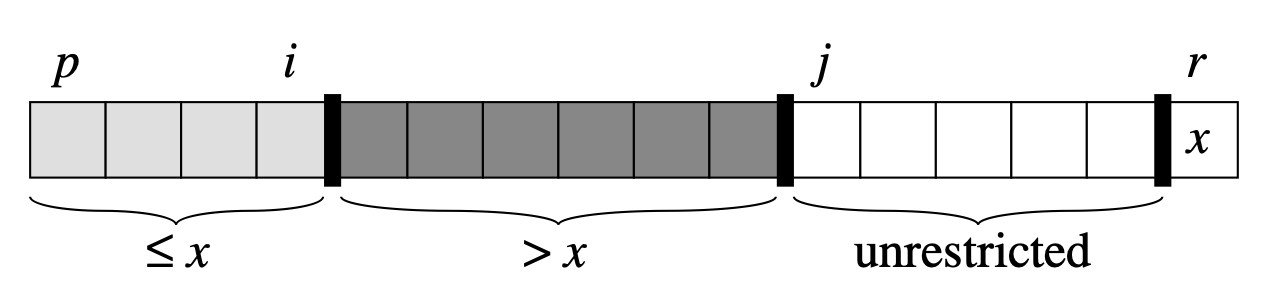
\includegraphics[width=10cm]{partitions}
	\caption{Partitions in a Quicksort}\label{fig:quick}
\end{figure}

\subsection{Merge Sort}

Merge sort is another recursive algorithm that divides an array into subarrays, sorts them recursively and merges the resulting subarrays into an end result. This procedure relies on a \textsc{Merge} function that compares two stacks element-by-element and merges them by placing the smaller of two elements into the result stack first. This comparison is then done recursively on ever-smaller subarrays, until the subarray length is one. In order to simplify code, the version below places \emph{Sentinels} at the end of subarrays to terminate the comparison process and not have to track how many elements have been compared.

\begin{algorithm}
	\caption{Merge Sort}\label{alg:merge}
	\begin{algorithmic}
		\Function{Merge-Sort}{\emph{A,p,r} }
		\If{\( p < r \) }\Comment{Check if the array is longer than 1}
		\State{\( q \leftarrow \lfloor\frac{p+r}{2}\rfloor \) }
		\State{\textsc{Merge-Sort}\( (A,p,q) \) }
		\State{\textsc{Merge-Sort}\( (A,q+1,r) \) }
		\State{\textsc{Merge}\( (A,p,q,r) \) }
		\EndIf{}
		\EndFunction{}
		\\
		\Function{Merge}{\emph{A,p,q,r} }
		\State{\( n_1 \leftarrow q-p+1 \) } \Comment{Length of left subarray}
		\State{\( n_2 \leftarrow r-q \) } \Comment{Length of right subarray}
		\State{let \( L[1 \ldots n_1 + 1] \) and \( R[1 \ldots n_2 + 1] \) be new arrays  } \Comment{Extend length by 1 for sentinels}
		\For{\( i = 1 \)  \textbf{ to } \( n_1 \) } \Comment{Copy left subarray}
		\State{\( L[i] \leftarrow A[p+i-1]\) }
		\EndFor{}
		\For{\( j = 1 \)  \textbf{ to } \( n_2 \) } \Comment{Copy right subarray}
		\State{\( R[j] \leftarrow A[q+j]\) }
		\EndFor{}	
		\State{\( L[n_1 + 1] \leftarrow \infty \) } \Comment{Insert sentinels}
		\State{\( R[n_2 + 1] \leftarrow \infty\) }
		\State{\( i \leftarrow 1 \) }
		\State{\( j \leftarrow 1 \) }
		\For{\( k = p \) \textbf{ to } r }
		\If{\( L[i] \leq R[j]\) } \Comment{Pick left element}
		\State{\( A[k] \leftarrow L[i]\) }
		\State{\( i \leftarrow i + 1 \) }
		\Else{ \( A[k] \leftarrow R[j] \)} \Comment{Pick right element}
		\State{\( j \leftarrow j+1 \) }
		\EndIf{}
		\EndFor{}
		\EndFunction{}
	\end{algorithmic}
\end{algorithm}

\subsection{Summary of Sorting and Search Algorithms}
The worst-case and average-case time complexities are shown in 

\begin{table}[H]
	\centering
	\begin{tabular}{@{}lll@{}}
	\toprule
	\textbf{Algorithm}  & \textbf{Worst Case}  & \textbf{Average Case} \\ \midrule
	Bubble Sort & \( \mathcal{O}(n^2) \) & \( \Theta(n^2) \) \\
	Insertion Sort & \( \mathcal{O}(n^2) \) & \( \Theta(n^2) \) \\
	Quick Sort & \( \mathcal{O}(n^2) \) & \( \Theta(n \log(n)) \) \\
	Merge Sort & \( \mathcal{O}(n \log(n)) \) & \( \Theta(n \log(n)) \) \\
	Linear Search & \( \mathcal{O}(n) \) & \( \Theta(n) \) \\
	Binary Search &\( \mathcal{O}(\log(n)) \) & \( \Theta(\log(n)) \) \\
	\bottomrule
	\end{tabular}
	\end{table}

\section{Computational Complexity}
A procedure with exponential time-complexity will always be worse than polynomial time-complexity. This helps differentiate efficient from inefficient algorithms.

A problem can be viewed a set of inputs that satisfy some property outlined by the problem. A \textbf{complexity class} is a set of problems that can be solved with a specific complexity, i.e.\ a specific amount of computational resources.

Complexity classes \textbf{do not contain algorithms}; they contain inputs (or words). We can classify problems in terms of the algorithms used to solve them, but only the problems are in the same complexity class.

\subsection{Complexity Classes}
\paragraph{P} The class of problems that can be \textbf{solved}  in polynomial time \( \mathcal{O}(n^k) \) and can be considered ``easy'' in the sense that an efficient algorithm exists to solve them.

\paragraph{NP} The class of problems that can be \textbf{verified} (using a \emph{certificate} in the form or a result that can be checked)  in polynomial time but solved only in non-polynomial, i.e.\ exponential time.

\paragraph{NP-hard} The class of problems that are at least as hard as any problem in NP and with the property that any problem in NP can be reduced to the NP-hard problem, meaning it can be transformed and then solved, yielding the answer for both the NP-hard problem and the NP problem. Some of these problems extend beyond NP.

\paragraph{NP-complete} The class of problems that are both NP-hard and in NP.

NP-complete and NP-hard problems are unlikely to have a solution in polynomial time. It has not yet been proven to be impossible.

In an NP-complete problem, we need to check \emph{every} possible candidate solution which might be an exponential number of inputs to check. This is similar to linear search, which checks every element of a vector.



\end{document}

